%-------------------------------- Configurações --------------------------------

\documentclass[a4paper,         % Tamanho do papel: A4
	           abntfigtabnum,
	           noindentfirst,
	           normaltoc,
	           pnumplain,
	           notimes
	           % capchap,
]{abnt}

\usepackage[utf8]{inputenc}
\usepackage[brazil]{babel}
\usepackage{graphicx}
\usepackage[pdfborder={0 0 0}]{hyperref} % http://www.tug.org/applications/hyperref/manual.html
\usepackage[alf]{abntcite}
\usepackage{listings} % http://www.atscire.de/index.php?nav=products/listings2 http://linorg.usp.br/CTAN/macros/latex/contrib/listings/listings.pdf
\usepackage{textcomp}
\usepackage[usenames,dvipsnames]{xcolor} % http://en.wikibooks.org/wiki/LaTeX/Colors

\urlstyle{same} % http://en.wikibooks.org/wiki/LaTeX/Hyperlinks#Customization

%-------------------------------- Highligthing ---------------------------------

\lstset{
    language=ruby,
    basicstyle=\footnotesize\ttfamily,
    columns=flexible,
    numberbychapter=false,
    showstringspaces=false,
    frame=bottomline,
    tabsize=2,
    xleftmargin=17pt,
    framexleftmargin=17pt,
    framexrightmargin=5pt,
    framexbottommargin=4pt,
    numbers=left,
    numberstyle=\scriptsize\ttfamily\color{Gray},
    emphstyle=\color{OrangeRed},
    commentstyle=\color{Gray}\textit,
    stringstyle=\color{PineGreen},
    keywordstyle=\color{Blue},
    morekeywords={it, include, Given, When, Then, And, Scenario},
    morestring=**[s]{:}{\ }, % cheat para fazer o symbol parecer string
    morestring=**[s]{|}{|}, % cheat para fazer o |x| parecer string
    emph={Factory},
    % emph={[2]Funcionalidade, Como},
    % emphstyle=[2]\color{MidnightBlue},
 }

\usepackage{caption}
\DeclareCaptionFont{white}{\color{white}\footnotesize\bfseries}
\DeclareCaptionFormat{listing}{\colorbox{BrickRed}{\parbox{\textwidth}{#1#2#3}}}
\captionsetup[lstlisting]{format=listing,labelfont=white,textfont=white}

% Renomear listing e listings -> código e códigos
\renewcommand*\lstlistingname{Código}
\renewcommand*\lstlistlistingname{Lista de Códigos}

%--------------------------------- Informações ---------------------------------

\begin{document}

\titulo{Técnicas emergentes de desenvolvimento de software}
\autor{Hugo Henriques Maia Vieira}
\instituicao{Universidade Estadual do Norte Fluminense Darcy Ribeiro}
\orientador[Tutor: ]{Rodrigo Soares Manhães, M.Sc.}
\comentario{Monografia apresentada ao Curso de Graduação em Ciência da
Computação da Universidade Estadual do Norte Fluminense Darcy Ribeiro como
requisito para obtenção do título de Bacharel em Ciência da Computação, sob
orientação da Prof. Rodrigo Soares Manhães, M.Sc.}
\local{Campos dos Goytacazes/RJ}
\data{2011}


\capa
\folhaderosto

\begin{titlepage}
 \vspace*{5cm}
 \begin{flushright}
  ``As pessoas boas devem amar seus inimigos''\\\textit{Seu Madruga}
  \vspace{1cm}
 \end{flushright}
\end{titlepage}


\begin{center}
\textbf{AGRADECIMENTOS} \\ [2.5cm]
\end{center}

A meu pai, minha mãe e especialmente a você.



\listoffigures
\lstlistoflistings

\begin{resumo}
Aqui entra o resumo do meu trabalho que será a última coisa a ser feita.
\end{resumo}

\sumario

\chapter{Introdução}

O desenvolvimento de software passou, e de certa forma ainda passa, por uma fase conhecida como \emph{crise do software}, termo utilizado pela primeira vez por \citeonline{HumbleProgrammer}. A Engenharia de Software surgiu \cite{NaurRandell} numa tentativa de contornar esta crise. No entanto, a ela foi baseada em algumas considerações equivocadas, que serão abordadas posteriormente, fazendo com que falhasse na sua tentativa de contornar tal crise.

Com o passar dos anos, o mercado demanda e espera software inovadores e de alta qualidade, que sejam adequados a suas necessidades – e o mais rápido possível \cite{TheBusinessOfInnovation}. Como isso não foi praticável através do Engenharia de Software tradicional, buscou-se uma abordagem alternativa.

O desenvolvimento ágil de software, que neste ano de 2012 completa 11 anos, foi elaborado \cite{AgileManifesto} para resolver esta crise que a Engenharia de Software tradicional não conseguiu, focando nas pessoas ao invés do processo e abraçando as mudanças ao invés de evitá-las. De acordo com \citeonline{PMNetworkFailureDrop}, o \textit{Chaos Manifesto 2011}\footnote{O \textit{Chaos Manifesto} é uma pesquisa bienal realizada pelo \textit{The Standish Group} e teve início em 1994. As pesquisas publicadas em um ano representam os dados do ano anterior.} mostra que os resultados de 2010 representam, desde sua primeira edição, a maior taxa de sucesso nos projetos de desenvolvimento de software, que aumentou de 32\% em 2008 para 37\% em 2010. Segundo \citeonline{ResumoChaosReport}, o \textit{The Standish Group} conclui que uma das principais razões para o aumento da taxa de sucesso foi a utilização das metodologias ágeis, que cresce a uma taxa de 22\% CAGR\footnote{\href{http://en.wikipedia.org/wiki/Compound_annual_growth_rate} {Compound annual growth rate}} e hoje são adotados em 9\% de todos os projetos de TI em andamento e em 29\% dos novos projetos.

Como o desenvolvimento ágil é relativamente novo, diversos métodos e técnicas vem sendo desenvolvidos tendo como base os princípios e valores ágeis \cite{BDDRodrigo}. Sendo técnicas emergentes, ainda são pouco discutidas no meio acadêmico, este trabalho pretende contribuir com esta discussão e, de certa forma, com a introdução de técnicas vindas do mercado na academia.


\section{Objetivos}

O objetivo principal do presente trabalho é contribuir com a introdução de técnicas e discussões surgidas no mercado para a academia, além de compilar informações, hoje dispersas, sobre as vantagens e desvantagens da utilização de tais técnicas.

Existem também algumas questões em aberto no desenvolvimento ágil de software, que serão alvo de discussão neste trabalho.

\section{Metodologia}

Será feita uma explanação sobre cada técnica e uma discussão mostrando onde são melhor aplicadas, comparando as diferentes abordagens para cada técnica, bem como as vantagens e desvantagens em seu uso.

Como base para a discussão, será utilizado o kanban-roots\footnote{\url{http://github.com/hugomaiavieira/kanban-roots}}, que está sendo desenvolvido em conjunto com o presente trabalho.

O kanban-roots é um kanban\footnote{O termo tem origem no sistema Toyota de produção, onde kanban é a maneira como é coordenado o fluxo de peças na cadeia de suprimentos  \cite{AMaquinaQueMudouOMundo}. No contexto do presente trabalho, kanban é um quadro para visualização do fluxo de trabalho (tarefas) em um projeto.} online para auxiliar a organização e acompanhamento das tarefas em um projeto. O kanban-roots já está em produção e vem sendo testado e utilizado com sucesso por algumas pessoas e empresas, não só do Brasil, mas também da França, Lituânia, Polônia, Africa do Sul, Rússia, Inglaterra, China, Finlândia, Peru, Estados Unidos, entre outros.

Na figura \ref{img:tela_kaban_roots} pode ser visto um \textit{print} da tela do kanban de um projeto no kanban-roots.

\begin{figure}[h]
  \center
  \caption{Tela do kanban de um projeto no kanban-roots}
  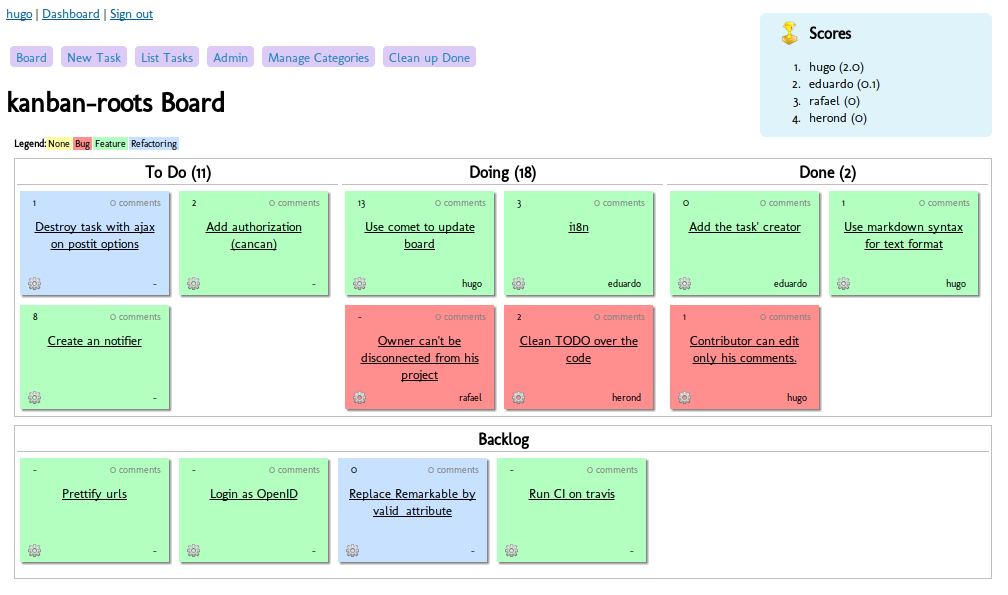
\includegraphics[scale=0.45]{images/kanban-roots}
  \label{img:tela_kaban_roots}
\end{figure}

Todos os trechos de código apresentados neste trabalho são trechos retirados do kanban-roots. A primeira linha de cada trecho sempre é um comentário informando o nome do arquivo original.

\section{Ferramentas}

Para o desenvolvimento do kanban-roots foram utilizadas diversas ferramentas, sendo importante citar em que contexto e momento cada uma delas é utilizada.

Como base para o desenvolvimento, foi utilizado o \textit{framework web} \textit{Ruby On Rails}\footnote{\url{http://rubyonrails.org}}. Para os testes de unidade apresentados na seção \ref{sec:tdd} foi utilizado o \textit{Test::Unit}\footnote{\url{http://test-unit.rubyforge.org/}}. Já na seção \ref{sec:bdd} é utilizado o \textit{Rspec}\footnote{\url{http://rspec.info/}} para testes unitários, testes de aceitação e dublês de teste. Ainda na seção \ref{sec:bdd} também foi utilizado o \textit{Cucumber}\footnote{\url{http://cukes.info/}} para testes de aceitação. Além dessas ferramentas, também foi utilizado o \textit{FactoryGirl}\footnote{\url{https://github.com/thoughtbot/factory_girl}} para \textit{fixtures replacement} em todos os momentos em que se fez necessário.
\chapter{Fundamentação teórica}

\section{Agilismo}
\label{sec:agilismo}

Em 2001 um grupo de dezessete especialistas, reconhecidos pela comunidade como grandes nomes do desenvolvimento software, se reuniram para discutir sobre um crescente conjunto de métodos que vinham surgindo e decidiram usar o termo Agilismo para descrever essa nova geração de métodos ágeis \cite{AgileStory}. Na mesma reunião, eles também escreveram o Manifesto Ágil \cite{AgileManifesto}, delineando um conjunto de valores e princípios que, em resumo, trilham um caminho para a eliminação de documentação e processos desnecessários, buscando a simplicidade, com foco na geração de valor e proximidade com o cliente, além de possibilitar respostas rápidas e eficazes às mudanças.

Pode-se dizer então, que o Desenvolvendo Ágil, ou Agilismo, é um rótulo genérico para os métodos de desenvolvimento de software baseados no Manifesto Ágil \cite{BDDRodrigo}.

% section agilismo (end)

\section{Tipos de teste}
\label{sec:tipos_de_teste}

\subsection{Testes de unidade}
\label{sub:testes_de_unidade}

Testes de unidade são testes nos quais unidades individuais do sistema são testadas para determinar se estão aptas para uso. Uma unidade é a menor parte testável de uma aplicação. Em programação procedural uma unidade pode ser uma função ou \textit{procedure}. Já em programação orientada a objetos, uma unidade pode ser um método.

% subsection testes_de_unidade (end)

\subsection{Testes de integração}
\label{sub:testes_de_integracao}

Teste de integração testam as integrações do código com o mundo exterior. Podem ser um teste que se comunique através da rede, tenha contato com o sistema de arquivos ou deixe os limites de seu próprio processo \cite{ArtOfAgileDevelopment}.

% subsection testes_de_integracao (end)

\subsection{Testes de aceitação}
\label{sub:testes_de_aceitacao}

Testes de aceitação são especificações para o comportamento e funcionalidade de um sistema. Os testes de aceitação nos mostram se o sistema se comporta corretamente pela perspectiva de um usuário, sem nos dizer nada sobre como o sistema implementa esse comportamento \cite{TestDrivenKoskela}.

% subsection testes_de_aceitacao (end)

% section tipos_de_teste (end)

%--------------------------------- Bibliografia --------------------------------

\citeoption{abnt-repeated-author-omit=yes}
\bibliographystyle{abnt-alf}
\bibliography{bibliografia}

\end{document}